

\documentclass{article}
%\usepackage[margin=1in]{geometry}
\setlength\topmargin{0pt}
\addtolength\topmargin{-\headheight}
\addtolength\topmargin{-\headsep}
\setlength\oddsidemargin{0pt}
\setlength\textwidth{\paperwidth}
\addtolength\textwidth{-2in}
\setlength\textheight{\paperheight}
\addtolength\textheight{-2in}

\usepackage[english]{babel}
\usepackage[utf8]{inputenc}
\usepackage{fancyhdr}
\usepackage{listings}
\usepackage{graphicx}
\usepackage{xcolor}


\definecolor{codegreen}{rgb}{0,0.6,0}
\definecolor{codegray}{rgb}{0.5,0.5,0.5}
\definecolor{codepurple}{rgb}{0.58,0,0.82}
\definecolor{backcolour}{rgb}{0.95,0.95,0.92}


\usepackage{booktabs}
\usepackage{pgfplotstable}



\lstdefinestyle{mystyle}{
	backgroundcolor=\color{backcolour},   
	commentstyle=\color{codegreen},
	keywordstyle=\color{magenta},
	numberstyle=\tiny\color{codegray},
	stringstyle=\color{codepurple},
	basicstyle=\ttfamily\footnotesize,
	breakatwhitespace=false,         
	breaklines=true,                 
	captionpos=b,                    
	keepspaces=true,                 
	numbers=left,                    
	numbersep=5pt,                  
	showspaces=false,                
	showstringspaces=false,
	showtabs=false,                  
	tabsize=2
}
\lstset{style=mystyle}


% header
\pagestyle{fancy}
\fancyhf{}
\rhead{CS 491}
\lhead{Pedram Safaei and Kevin Carlos}
\rfoot{Page \thepage}
\usepackage{listings}

\begin{document}
	\section{Nearest Neighbor}
	\subsection{Describe Implementation}
	The general idea is to compute the L2 Norm to the nearest neighbor, K point, and return the most recurring label in those neighbors.
	
	\subsubsection{KNN\_TEST}
	This function genrates a label based on the points given to it, computes the distance, to each of those points (training points) and puts them in a list. This list is then sorted based on the distance that was calculated before. The subset of the K nearest neighbor or point will have their labels summed and then we will output the sign of the summation as the label, so if our predicted label is less than 0 we return -1 and if it is greater than 0 we return 1. In case the predicted value is 0 we will choose the result based on the ordering of the training data and from the set of neighbors in the sorted list.
	\begin{lstlisting}[language=Python]
	def KNN_test(X_train, Y_train, X_test, Y_test,K):
		NumberOfCorrect = 0
		for i, j in enumerate(X_test):
			radius = []
			for n, m in enumerate(X_train):
				radius.append(((math.pow((m[0] - j[0]), 2) + math.pow((m[1] - j[1]), 2)), Y_train[n][0]))
		List_sorted = sorted(radius, key=lambda member: member[0], reverse=False)[:K] 
		predictedvalue = sum([member[1] for member in List_sorted])
		if (not predictedvalue):
			predictedvalue = List_sorted[0][1]
		elif (predictedvalue < 0):
			predictedvalue = -1
		elif (predictedvalue > 0):
			predictedvalue = 1
		if predictedvalue == Y_test[i][0]:
			NumberOfCorrect = NumberOfCorrect+1
		return NumberOfCorrect / len(X_test)
	\end{lstlisting}
	
	\subsubsection{Choose\_K}
	This function is simply checking all possible accuracies on the given test data and returns the index with the greatest accuracy which will be our K.
	\begin{lstlisting}[language=Python]
		OldAccuracy = 0
		NewAccuracy = 0
		Predicted_K = 1
		K = len(X_train)
		for i in range(1, K):
			OldAccuracy = KNN_test(X_train,Y_train,X_val,Y_val, i)
			if(OldAccuracy>NewAccuracy):
				NewAccuracy = OldAccuracy
				Predicted_K = i
		return Predicted_K
	\end{lstlisting}
	\subsection{Algorithm Classification}
	
	Using the testing data given to us from the project description we will get the following results 
\begin{center}
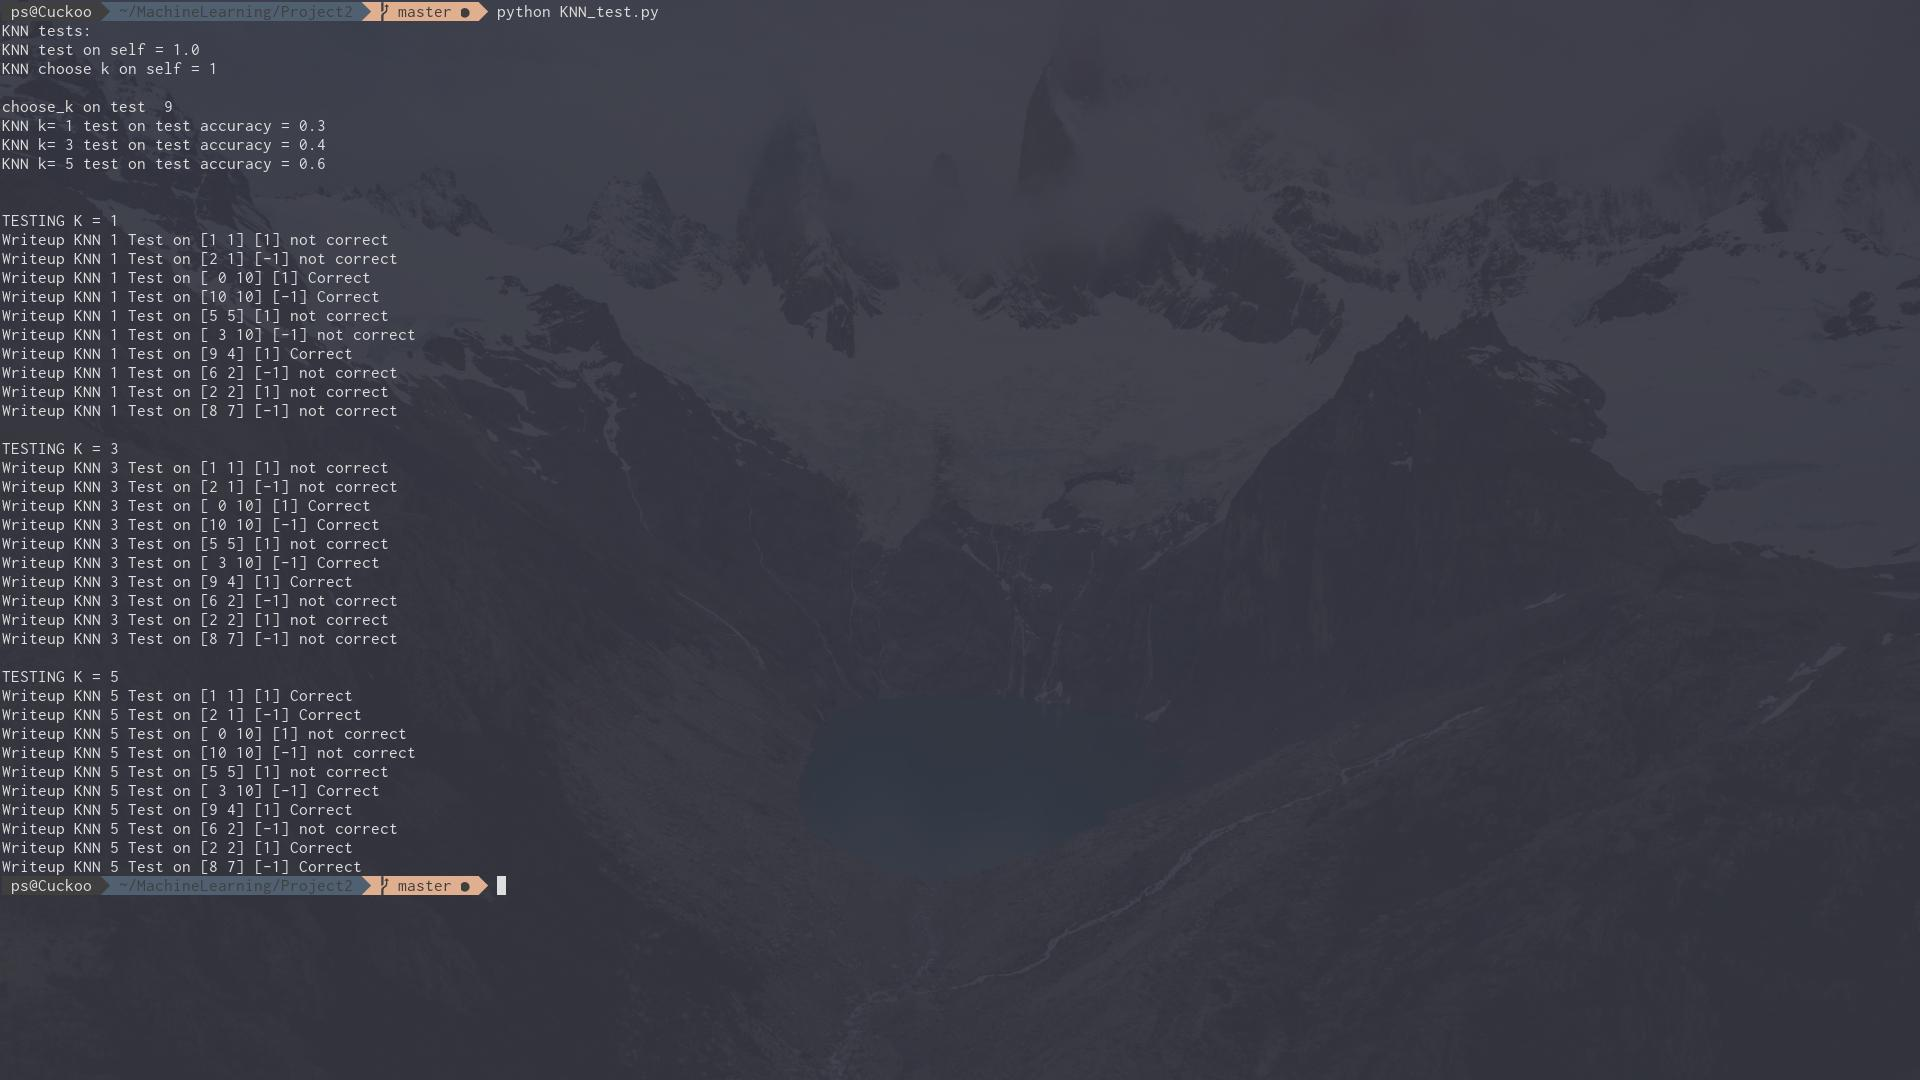
\includegraphics[scale=.24]{KNN.jpg}
	\footnote{The picture has a high resolution so you should be able to zoom in and see the detail, but the picure has also been included in the zip file so please refer to that if there is any issues}
	
\end{center}
	The best K for our Algorithm would be 9 with the accuracy of 0.7
	\begin{center}
		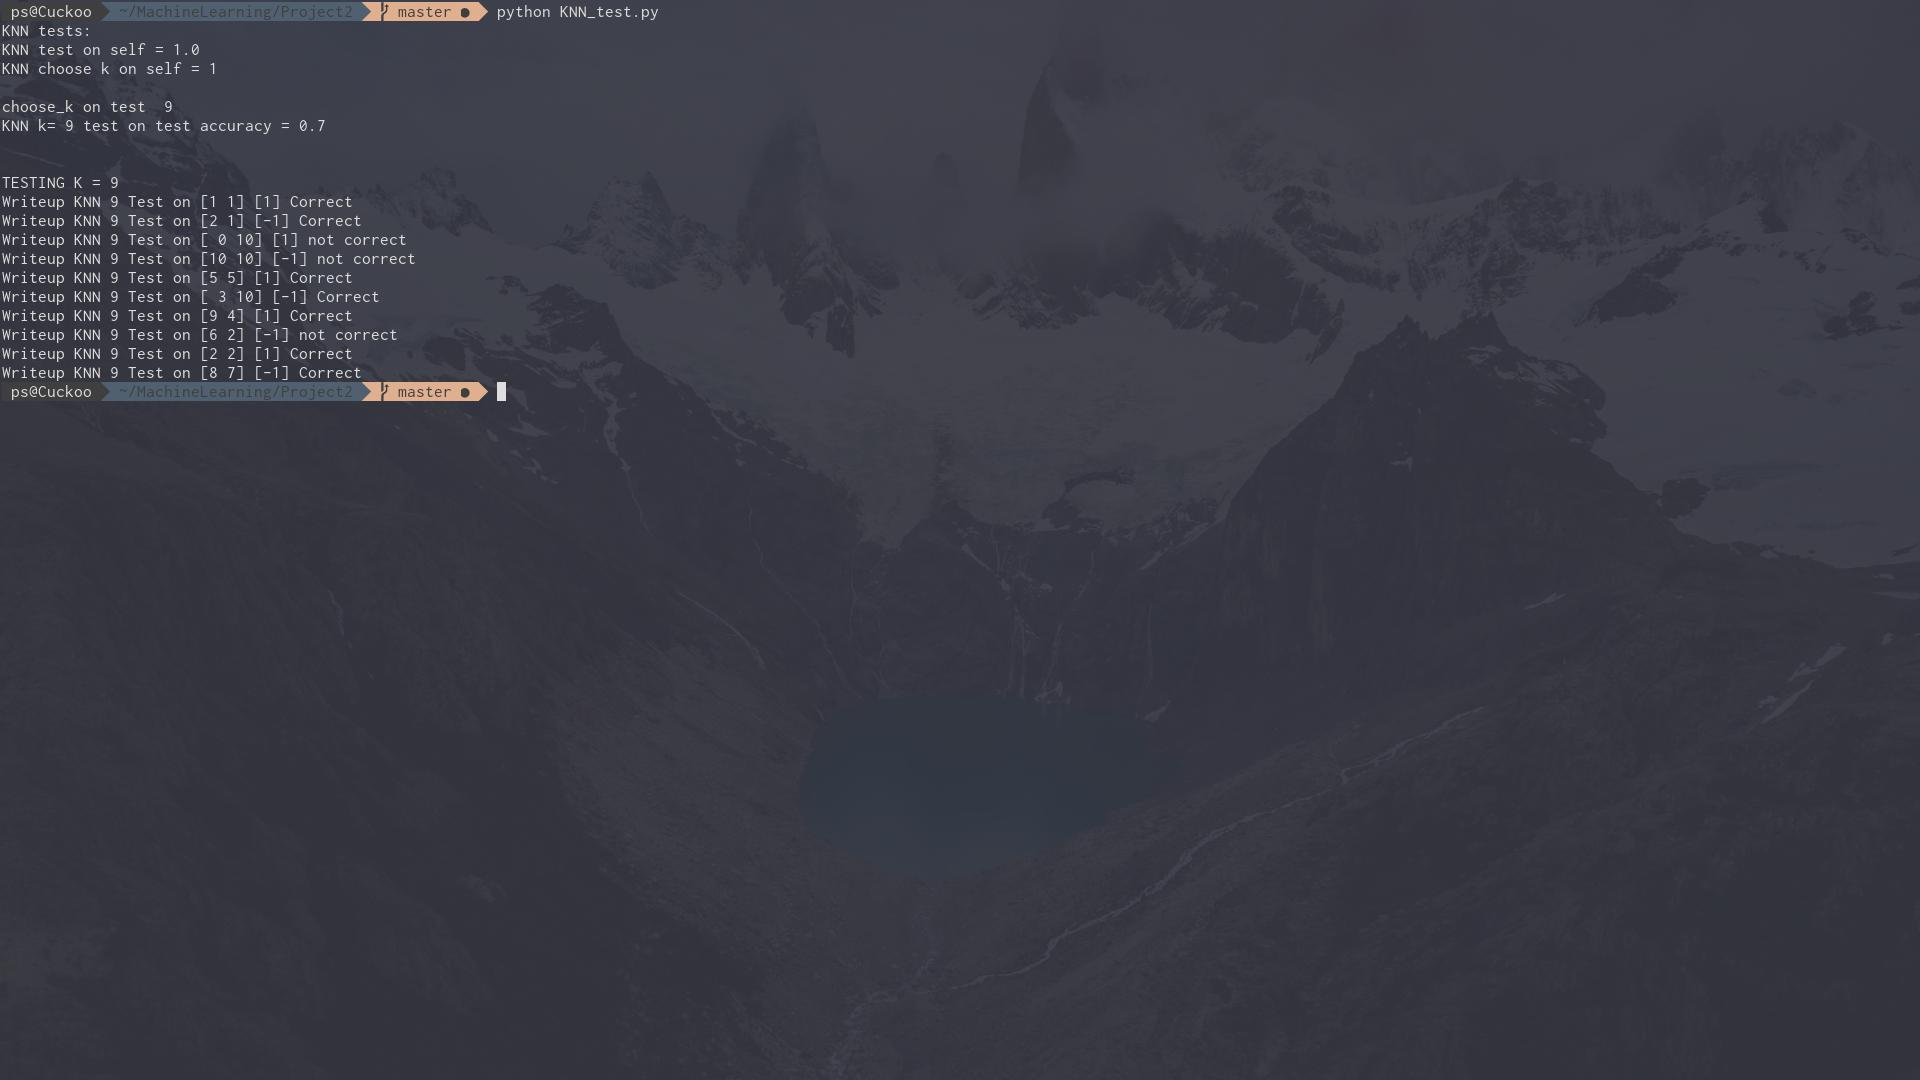
\includegraphics[scale=.24]{KNN2.jpg}
		\footnote{The picture has a high resolution so you should be able to zoom in and see the detail, but the picure has also been included in the zip file so please refer to that if there is any issues}
		
	\end{center}

	\section{Perceptron}
	\subsection{Describe Implementation}
	\subsection{Decision Boundary}

\end{document}


